\documentclass{article}
\usepackage[utf8]{inputenc}
\usepackage[portuges]{babel}
\usepackage{graphicx}
\usepackage{index}
\renewcommand{\baselinestretch}{1.50}\normalsize
\renewcommand{\paragraph}{%
  \@startsection{paragraph}{4}%
  {\z@}{3.25ex \@plus 1ex \@minus .2ex}{-1em}%
  {\normalfont\normalsize\bfseries}%
}
\parskip 7.2pt
\parindent 8pt

\newfloat{figure}{thp}{lop}
\floatname{figure}{Figure}

\begin{document}


\begin{titlepage}
    \begin{center}
        {\large INSTITUTO FEDERAL DE EDUCAÇÃO, CIÊNCIA E TECNOLOGIA DO RIO GRANDE DO SUL } \\
        {\large CÂMPUS BENTO GONÇALVES-RS} \\[4.9cm]
        {\large Jean Carlo Machado} \\[4.9cm]
        {\Huge Criação de Jogos Digitais com HTML5} \\[4.9cm]
        \vfill
        {\large Bento Gonçalves, Julho 2013} 
    \end{center}
\end{titlepage}

% Folha de rosto sem o uso de \folhaderosto
\begin{titlepage}
    \begin{center}
        {\large Jean Carlo Machado} \\[2.3cm]
         {\Huge Criação de Jogos Digitais com HTML5 } \\[2.3cm]
        {\large Trabalho de conclusão de curso} \\[2.3cm]
        \hspace{.45\textwidth} % posicionando a minipage
        \begin{minipage}{.5\textwidth}
            \begin{espacosimples}
                Projeto de Pesquisa apresentado junto ao Curso de Tecnologia em Análise e Desenvolvimento de Sistemas do Instituto Federal de Educação, Ciência e Tecnologia do Rio Grande do Sul, como requisito parcial ao desenvolvimento do Trabalho de Conclusão de Curso. 
                \\\\Orientador: Dr. Rogério Tessari
            \end{espacosimples}
        \end{minipage}
        \vfill
        {\large Bento Gonçalves, Julho 2013} 
    \end{center}
\end{titlepage}

\vfill
\setlength{\ABNTsignthickness}
\assinatura{}
\assinatura{}
\assinatura{}
\end{folhadeaprovacao}
\newpage

\listoffigures  
\listoftables
\newpage

\tableofcontents
\newpage

\section{CONTEXTUALIZAÇÃO}
\subsection{História e benefícios dos jogos}
\indent Há muito os jogos são utilizados como meio de entretenimento, mas além da diversão, estes podem ser benéficos de diversas outras formas, como apuração da capacidade lógica, desenvolvimento do trabalho em equipe, etc.

\\mais beneicios de jogar
\\
Na informática os jogos estão presentes desde meados dos anos 60, no início eram extremamente simples e totalmente dependentes da plataforma onde eram desenvolvidos, sem mencionar o fato de serem protótipos de laboratório os quais nunca sairam destes locais. 
\\
Com a criação da Atari em 1972, os jogos eletrônicos se popularizaram criando um mercado competitivo onde grandes corporações internacionais disputavam para criar as melhores plataformas (consoles) e jogos.  Essas corporações dentre as maiores  ressalta-se: Nintendo, Sony e Microsoft; devido ao alto nível de competitividade do mercado desenolveram novas tecnologias afim de se destacar criando novos conceitos e aumentando o entretenimento e imersão do usuário. Exemplos destas tecnologias são: renderizadores de elementos de 3 dimensões (3D), bibliotecas de física avançada, produções musicais específicas para os jogos, bem como o acréscimo no nível de detalhamento gráfico devido às GPU's \textit{Graphics Processing Unit's} (ou unidades de processamento gráfico) mais poderosas utilizadas. 
\\
Segundo (BUCHMAN,1996) \begin{quote} A indústria dos videogames foi rejuvenescida com a introdução da Nintendo ao final nos anos 80. Com melhoras significativas  nos gráficos, no realismo e com a introdução de jogos violentos, a Nintendo conseguiu uma dominância de mercado temporária.
\end{quote}

O mercado global de jogos cresceu de 70.5 billões de dólares em 2011 e espera chegar a 117.9 bilhões em 2015, crescendo em méia 13.7 por cento de 2011 a 2015 (AK, 2012).
Ainda segundo (AK,2012) \begin{quote} A disponibilide de internet de alta velocidade, a sofisticação das técnicas dos jogos, e a grande compatibilidade dos hardwares, aumenta o fluxo de entrada de dinheiro, o que está gerando um grande \textbf{boom} na indústria dos jogos.\end{quote}

\begin{figure}[!htbp]
    \begin{center}
        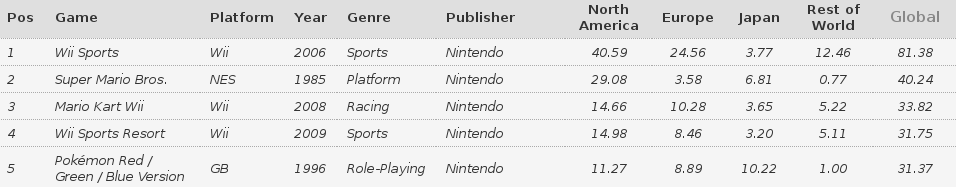
\includegraphics[width=\textwidth]{bestSelledGames.jpg}
               \caption{Os cinco jogos mais bem vendidos de todos os tempos segundo à VGChartz, 2013) . \label{fig:Jogos mais bem vendidos}}
    \end{center}
\end{figure}

Além de obter uma estimativa de vendas dos jogos mais populares, através desta lista é possivel ter-se uma concepção de quais gêneros de jogos atrem mais os usuário. O gênero de maior influência na lista é o de esportes, seguido igualmente por plataforma, corrida e RPG.
\footnote{A VGChartz é uma bem conceituada   empresa na área de pesquisas de mercado especificamente de jogos eletrônicos.}

\subsection{Tendência smart devices}

Atualmente, principalmente devido ao baratemento e miniaturalização dos componentes, tendência prevista por Moore em 1965, bem como a massificação da internet, o advento dos smart devices está em plena ascenção. 

\newpage

\begin{figure}[!htbp]
    \begin{center}
        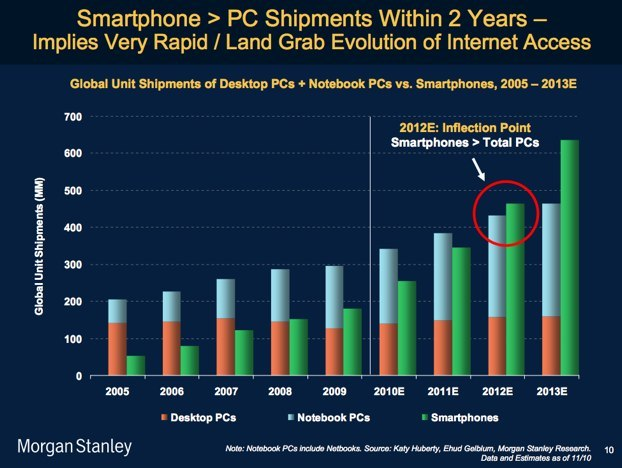
\includegraphics[width=\textwidth]{smartvscomputer.jpg}
               \caption{Previsão de vendas de smartphones vs pc's}
    \end{center}
\end{figure}

\footnote{(WEINTRAUB, 2012) mostra que esta previsão se tornou realidade no último trimestre de 2010.}

Smart devices são dispositivos que anterioremente serviam para um propóstito específico, os quais tiveram poder de processamento e recursos similares aos dos computadores pessoais agregados. Os smart devices geralmente possibilitam conectar-se a internet, instalar e remover programas, rodar aplicativos que demandam alto teor de processamento como jogos, vídeos, entre outros recursos. São exemplos de smart devices: smart-phones, smart-tablets e smart-tv's.

 Devido a estes dispositivos rodarem em micro-processadores comuns e ao alto nível de abstração dos sistemas operacionais atuais, migrá-los para os sistemas operacionais atuais é uma tarefa relativamente trivial. Um exemplo desta convergência é o Ubuntu da Canonical e o Windows Phone da Microsoft, os quais já rodam em praticamente todos os tipos de smart devices. Isso permite a migração de grande parte dos aplicativos desenvolvidos para os computadores (Desktop) para os smart devices, agregando assim, além de seus benefícios primevos, os trunfos que cada plataforma específica pode oferecer.
 \\
 Contudo, com a grande popularização dos smart devices, principalmente os smart-phones, cada vez mais novos sistemas operacionais para estes dispositivos fazem-se disponíveis, cada qual com particularidades tais como linguagens suportadas, recursos mínimos e aparelhos compatíveis, são exemplos de sistemas operacionais para smart-phones: Android, FirefoxOS, Ubuntu, IOS, Windows Phone e o ainda não lançado Taizen. Sob esta perspectiva os desenvolvedores sentem cada vez mais o desafio que é construir aplicativos com abrangência suficiente de plataforma, de modo a alcançar todos ou a grande maioria de seus usuários. 
\\
 \\
 Outro desafio, não menos importante, é tornar a experiência dos usuários através destas plataformas e dispositivos o mais transparente o possível, pois não é expectativa do usuário ter que reapreder a utilizar um aplicativo simplesmente por ter trocado de aparelho, outrossim, uma experiência muito mais compensadora seria se o aplicativo adapata-se suas diferenças, mas somente estas, legando ao restante da aplicação uma experiência idêntica. Dessa forma seria possível que o aplicativo, uma vez instalado, se comportasse exatamente como o mesmo em cada dispositivo, sendo possível um usuário deixar de fazer algo em X e continuá-lo do mesmo ponto em Y, uma arquitetura assim permitiria que os dispositivos fossem transparecidos, possibilitando ao usuário fazer a troca entre dispositivos de acordo com o benefício de utilização que cada plataforma provê, Por exemplo, um usuário em um ônibus, jogaria um jogo em seu celular ou tablet, acho chegar em seu destinho, utilizaria de seu laptop, quando em casa utilizaria de sua smart-tv.

 Tratando-se de jogos, o desafio deste tipo de proposta é ainda maior, pois este tipo de aplicação é intrínssicamente mais difícil de construir e geralmente fazem uso de recuros que não estão disponíveis em outras plataformas como por exemplo: geolocalização (dispível em dispositivos móveis, mas não em smart-tv's e computadores pessoais), acelerômetro (o mesmo que geolocalização), etc. 

\subsection{O jogo}

Sob esta perspectiva, este projeto propõe  a criação de um jogo em HTML5, de estilo plataforma, que englobe e proporcione uma forma de contornar os problemas acima mencionados, provendo assim, uma experiência para o usuário final o mais transparente de plataforma o possível, mesmo utilizando de recursos específicos de plataforma.

, entendendo plataforma por: um jogo de aventura 2D onde o personagem com o objetivo de chegar ao outro lado do mapa, enfrentando desafios de terreno, bem como oponentes, Cabendo por parte do jogador, resolver os problemas lógicos que o cenário propõe e conduzir o personagem com agilidade pelos obstáculos. Caso o personagem venha a morrer (através de buracos, terrenos inapropriados ou inimigos) o usuário deverá recomeçar o jogo. 

\\melhorar
Através de um jogo o projeto busca mostrar se é possível a construção de aplicativos independetes de plataforma fornecam uma sensação de continuidade ao trocar de um dispositivo para outro. Um caso de uso explanatório seria basicamente o seguinte: Um usuário começa o jogo em seu laptop enquanto fora de casa, sem seu trajeto joga no seu smartphone e ao chegar em casa o utiliza em sua smart-tv.

\section{PROBLEMA}

Desenvolverdores tem dificulade em criar aplicativos que ofereçam transparência de plataforma em dispositivos de diferentes tipos, como computadores, smartphones e smarttv's. O problema se dá, principalmente, devido à alta gama de plataformas e as diferenças de arquitetura destas. Acarretando assim, na segmentação de aplicativos por plataformas, ou então na construção de um aplicativo para cada plataforma alvo, aumentando muito o tempo de desenvolvimento e o custo de produção. Esta situação agrava-se ainda mais quando relativo aos jogos, devido à intrínsseca dificuldade de desenvolvimento deste tipo de software. 

\section{OBJETIVOS}
\subsection{Objetivo primário}

Desenvolver uma única versão de um jogo de plataforma o qual a troca do tipo de dispositivo (smartphone, smartv's e computadores) seja transparente, ou seja, que  permita ao usuário alternar entre arquitetura durante uma partida e continuar seu jogo onde parou mesmo fazendo uso de características peculiares de cada dispositivo afim de oferecer a melhor experiência possível de acordo com a plataforma de utilização.

\subsection{Objetivos secundários}

Dentre os objetivos de caráter secundários constam:

\begin{itemize}
\item Verificar o quanto cada um dos seguintes quesitos pode ser atendido em cada plataforma e quais as customizações necessárias para atendê-lo: movimentação;
\item Identificar as melhores formas de explorar a iteração nos diferentes tipos de dispositivos (formas de comandar as funcionaidades do jogo em cada tipo de dispositivo)
\item Deseja-se também identificar os pontos relevantes (fraquezas e acertos) da implementação atual do HTML5, em diferentes tipos de plataformas, dessa forma, sendo possível obter uma visão panorâmica de o quanto falta para esta tencologia estar plenamente estabelecida;
\item O estudo das seguintes tecnologias: html5 (especificamente canvas, àudio, vídeo e controle de entrada) , frameworks de desenvolvimento de jogos em HTML5, bibliotecas de detecção de recursos, tecnologias para preenchimento de gaps HTML5.
\end{itemize}

\section{JUSTIFICATIVA}

O trabalho justifica-se primeiramente pelo quesito inovação, devido ao HTML5 ser uma tecnologia não totalmente consolidada, sendo de útilidade à comunidade trabalhos que revisem seus recursos, quanto mais em escopos específicas como o HTML5 para a construção de jogos que utilizam de recursos específicos de dispositivos.

É justificável também por forncer uma nova forma de iteração com os jogos, fornecendo uma experiência transparente em relação à plataforma.

Este trabalho, devido à sua lincesa GLP, pode ser utilizado como base para o desenvolvimento de outros jogos que busquem horizontalidade entre plataformas.

Justifica-se também por fornecer uma revisão sobre o estado da arte das tecnologias que permitem a criação de aplicativos para dipositivos diferenciados.

Devido ao completo mapeamento do proceesso de desenvovimento de um jogo, este trabalho pode servir como um manual dos aspectos que devem ser observados para a criação de um jogo.

\section{REVISÃO BIBLIOGRÁFICA}
\subsection{HTML5}

O padrão HTTP é conhecido por ser o principal fomentador da WEB e a especificação de texto deste padrão é o conhecido HTML, em sua concepção inicial, Tim Berners-Lee acreditava que seria possível  interligar hipertextos em computadores diferentes com uso de links globais também chamados de hiperlinks (SILVA 2011).
\\
\\ Trata-se de uma linguagem de marcação que define a estrutura de elementos que uma página deve ter de modo a fornecer conteúdo iterativo aos usuários. Todavia, a iteratividade necessária para a construção de jogos animados em HTML é algo recente, anteriormente só se obtinha com a utilização de ferramentas proprietárias como o Adobe Flash, Microsoft Silverlight e Oracle JavaFX.  No HTML5 esta iteratividade é alcançada através da utilização do recurso canvas, que é a tag HTML que permite-se "desenhar"  dentro da página. 

\\Atualmente o canvas suporta somente o desenvolvimento 2D, sua implementação 3D está em desenvolvimento e chama-se WebGL. Por consequência do ainda baixo nível de especificação do WebGL, não optamos por o desenvolvimento de um aplicativo 3D.

O HTML5 por fatores como a excelente documentação, grande comunidade de desenvolvedores e usuários e por último mas não menos importante por seu caráter multiplataforma, justifica-se para a construção de jogos "transparentes". Segundo (KURYANOVICH, 2012) "a beleza de desenvolver jogos com o padrão aberto WEB é que este nos delega a escrever uma vez e utitilizar em qualquer lugar".

Apesar de a tecnologia  ainda não estar completa ela já demonstra grande robustez  e os padrões de desenvolvimento invariavelmente estão migrando para a perspectiva HTML5, segundo (TABUSCA, 2013) desenvolvedores que atualmente trabalham no ramo da Web, já podem visualizar que o novo ramo do desenvolvimento de aplicativos mobile está se aproximando mais e mais à elusiva proposta do HTML5.

\subsection{Motores de física}

Motores de física (\textbf{Engines de física}) provêm a um software, através de equações matemáticas, um modelo similar das leis da física, estes motores podem ser utilizados na construção de games, simuladores entre outros. As bibliotecas de física segundo (SHANKAR, 2012), "geralmente incluẽm os seguintes recursos: elasticidade, gravidade fricção e conservação de \textbf{momentum} entre dois ou mais objetos que colidem".

Dentre as bibliotecas mais populares que implementam física, compatíveis com HTML5 constam:

\begin{itemize}
\item box2dweb: é um port de sua versão em C++, desenvolvida exclusivamente para ambientes 2D, rica em opções e razoavelmente fácil de utilizar.
\item Ammo.js: baseada na biblioteca bullet para física 3D, tem um grande set de funcionalidades, todavia é razoavelmente mais compicada de utilizar.

\item JigLibJS: outro port de C++, todavia escrito à mão, com melhorias para o Javascript.  Segundo (PRALL), "à customização rendeu à JigLibJS extra performance se comparada ao Ammo.js, todavia esta não é tão rica em opçãoes."
\end{itemize}

\subsection{Frameworks para desenvolvimento de jogos HTML5}

enchant.js
three.js

\subsection{Environments para desenvolvimento HTML5}


Após esta revisão das ferramentas  e tecnologias disponíveis, fica claro que a utilização de cada uma delas para a criação de um jogo não é um processo trivial, foi pensando nisso que algumas empresas lançaram frameworks "full stack"  (ou framework de pilha completa) para a utilização destes tipos de recursos em mobile, interoperáveis. (JEFFRIES, 2012) define frameworks full stack relacionados ao desenvolvimento front-end como: "frameworks que nos auxiliam no completo desenvolvimento de uma aplicação, desde a interface com o usuário aos dados armazenados".

Na pesquisa efetuada sobre estes frameworks full stack foram identificadas as seguientes tecnologias:

\begin{itemize}

 \item segundo (PRADO, 2012) o GWT é um framework essencialmente para o lado do cliente (cliente-side) e dá suporte à comunicação com o servidor através de RPCs \textit{Remote Procedure Calls} (ou procedimento de chamadas remotas). Ele não é um framework para aplicações clássicas da web, pois deixa a implementação da
aplicação web parecida com implementações em desktop. Este é utilizado em muitos produtos de grande porte como o Google Adwords e Google Wallet. Outra característica interessante é que a plataforma opera sobre a licença Apache versão 2.
\item construct 2 
\item play canvas
\item CreateJS
 \item o ambiente  \textit{HTML5 Development Environment} (ou ambiente de desenvolvimento HTML5) da Intel, este fornece uma solução na nuvem, completa para o desenvolvimento em plataforma cruzada, com serviços de empacotamento, serviços para a criação e testes de aplicativos com montagem de interfaces drag and drop (Intex XDK) e biliotecas para a construção de jogos utilizando aceleração de hardware, o que garante até duas vezes mais performance que aplicativos mobile baseados em Web tradicionais. Esta solução é free, open source e funciona  através de um plugin para o Google Chrome, ou seja, o desenvolvimento também é multi-plataforma e devido ao fato de os binários ficarem hospedados na nuvem, possibilitou a  Intel criar compiladores para cada uma das plataformas disponibilizadas pelo PhoneGap, que é o framework polyfill utilizado na solução. 
\\\\
\end{itemize}

\subsection{Frameworks polyfill}

O HTML5 por não ser um padrão completamente especificado, deixa lacunas de suporte em plataformas, para recursos específicos tanto para a gestão de hardware quanto de software, acarretanda que muitos browsers não implementam algumas funcionalidades, completa ou parcialmente especificadas, daí surge a necessidade dos polyfills para implementar estas camadas.

Algumas tecnologias desta classe são:

\begin{itemize}
\item Suporte a SVG \textit{Scalable Vector Graphics} (ou vetor de gráficos escaláveis): svgweb, Raphael, canvg, fabric.js;
\item Suporte a \textit{Web Storage} (ou armazenamento na web): Amplify.js, storage polyfill, session storage;
\item Suporte a vídeo: video.js, SublimeVideo, html5media, LeanBack Player;
\item Suporte a Geo-localização: Webshims Lib, geolocaltion polyfill, GeoLocation-API-Polifill;
\end{itemize}

Uma das soluções mais promissoras polyfill é o PhoneGap ou Apache Cordova, esta ferramenta é open source e possibilita utilizar de inúmeros recursos de hardware da grande maioria das produtoras de dispositivos móveis.

\begin{figure}[!htbp]
    \begin{center}
        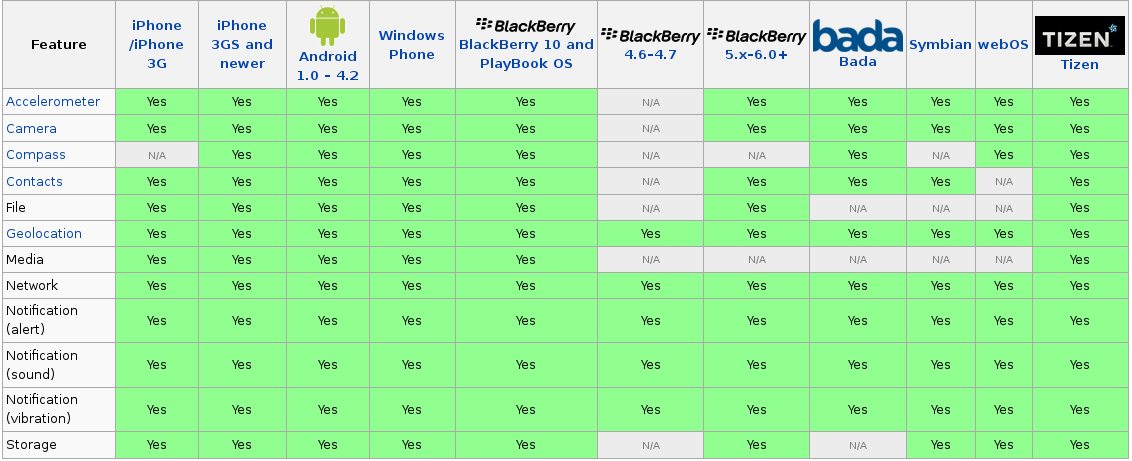
\includegraphics[width=\textwidth]{cordovaFeatures.jpg}
               \caption{Funcionalidades implementadas para o projeto Apache Cordova.\label{fig:Cordova}}
    \end{center}
\end{figure}

Segundo (JÚNIOR) utilizando as linguagens de desenvolvimento Web HTML, CSS e Javascript. Ele fornece um conjunto de APIs para acesso a funções nativas do Sistema Operacional e do hardware do dispositivo, utilizando Javascript. A proposta do PhoneGap é essencial para unir as especificidades de Web com detalhes de sistemas operacionais tanto de hardware como de software. 

\subsection{Som e vídeo}

\subsection{Entrada de comandos}

\subsection{Detecção de recursos}

Para detectar suporte aos mais variados recursos do HTML5 no browser do cliente existem duas possibilidades. Pode-se implementar testes para cada funcionaidade utilizada, abordando os detalhes de implmentação de cada uma, ou então fazer uso de alguma biblioteca especializada neste processo, Modernizr é uma opção open-source deste tipo de biblioteca, este gera uma lista de booleanos sobre grande variedade dos recursos HTML5, dentre estes, geolocalização, canvas, áudio, vídeo e local storage.

\subsection{Metodologia de desenvolvimento de software para a construção de games}

Como o jogo é um software complexo damanda-se a utilização de metodologias de engenharia de software, dentre os processos de software mais conhecidos, academicamente destacamos: 


\begin{itemize}
\item OpenUP: este é bem detalhado e de característica iterativa e incremental. Gerando assim, um levantamento mais apurado dos riscos, requisitos e outros detalhes do sistema e a criação incremental do sistema, com requisitos maleáveis.
\item Cascata: processo antigo, caracteriza-se por ser pouco maleável aos requisitos mapeados posteriormente ao processo de análise;
\item Processo ágil - SCRUM: sua utilização é flexível e sendo um método àgil especifica pouca documentação, ou como dizem, somente a documentação necessária, este processo é bem conhecido e aceito na comunidade de desenvolvimento de software.
\end{itemize}

// utilizar metodologia ágil (justificar) (artigo do rogério)
\subsection{Trabalhos similares} 

O browserquest da Mozilla é um jogo de RPG 8-bits focado em demonstrar na prática a utilização de muitos recursos do HTML5, este trabalho se assemelha razoavelmente ao browserquest, todavia, o browserquest não tem versão estável para a maioria dos dispositivos mobile e também distingue-se por não guardar algumas informações relativas ao estado como o posicionamento, impossibilitando assim, a experiência transparente proposta neste trabalho.

(SILVA,2010), demostra a utilização de HTML5 para a criação de jogos simples, todavia seu trabalho não se foca nas diferenças entre uma plataforma e outra. 

\section{METODOLOGIA}
//como vou  atingir os objetivos

Primeiramente há de ser criado uma versão demo utilizando de imagens e audio de características livre na internet, após o demo criado, pretende-se então construir os modelos reais, bem como selecionar as faixas musicais finais.

Para demonstrar se a horizontalidade proposta foi obtida, criar-se-à uma tabela comparativa que exponha as funcionalidades com características dependentes de plataforma, informando se o atendimento da funcionalidade obteve êxito e como se chegou a este resultado e quais outras soluções seriam possíveis.


\section{CRONOGRAMA}

O cronograma foi especificado de acordo com o detalhado na metodologia, suas datas estão especificadas de acordo com dias úteis disponíveis no calendário.\\
\begin{table}[!htbp]
                           \begin{center}
                \begin{tabular}{ | l | l | l | l | l |}
                \hline  
                \textbf{Identificador}& \textbf{Tarefa} &  \textbf{Duração} & \textbf{Início} & \textbf{Término} \\  \hline
                1 & Concepção & 5 dias & 1 agosto & 7 agosto \\  \hline
                2 & Elaboração & 15 dias & 8 agosto & 29 agosto \\  \hline
                3 & Contrução & 15 dias & 30 agosto & 19 setembro \\  \hline
                4 & Contrução & 10 dias & 31 agosto & 3 outubro \\ \hline
                  & Total & 45 dias & 1 agosto & 3 outubro \\
                \hline
                \end{tabular}
            \end{center}
               \caption{Cronograma do projeto. \label{fig:Cordova}}
\end{table}

\newpage 

\begin{thebibliography}{99}

\bibitem{KURYANOVICH2012}
  KURYANOVICH, Egor; SHALOM Shy, et all.
  \emph{The State of Open Web Games}.
  Addison Wesley, Massachusetts, pg. 12,
  ISBN: 978-1-4302-3978-9,
  2012.

\bibitem{SILVA2010}
SILVA, Jucimar Maria Júnior; FIRMINO, Emiliano Carlos M.
  \emph{Desenvolvimento de jogos em HTML5}.
  Coordenação da engenharia da Computação,
  Univerisdade Federal do Amazonas, 
  Amazonas, 2010.

  \bibitem{SILVA2010}
SHANKAR, Aditya Ravi .
  \emph{Pro HTML5 Games}.
 ISBN: 978-1-4302-4710-4, p. 39-64, 
 2012.  

 \bibitem{SILVA2010}
TABUSCA, Alexandru
  \emph{THE NEW “UNIVERSAL TRUTH” OF THE WORLD WIDE WEB}.
American University, School of Computer Science for
Business Management, Bucharest, 2013

 \bibliotecam{SILVA2010}
PRALL, Chandler 
  \emph{JavaScript Physics Engines Comparison}.
Disponível em: http://www.htmlgoodies.com/html5/client/javascript-physics-engines-comparison.html#fbid=AAlTVDXjb40
Acesso em: Jul 2013.
 
 \bibliotecam{AK2012}
AK, Sheela 
  \emph{ Global Gaming Market Is Expected to Reach USD 117.9 Billion by 2015: Transparency Market Research}.
Disponível em: http://www.prnewswire.com/news-releases/global-gaming-market-is-expected-to-reach-usd-1179-billion-by-2015-transparency-market-research-169284526.html
Acesso em: Jul 2012.

 \bibliotecam{VGChartz2013}
VGChartz
  \emph{Global sales (in millions of units) per game}.
Disponível em: http://www.vgchartz.com/gamedb/
Acesso em: Jul 2012.


 \bibliotecam{WEINTRAUB2012}
WEINTRAUB, Seth
  \emph{Industry first: Smartphones pass PCs in sales}.
Disponível em: http://tech.fortune.cnn.com/2011/02/07/idc-smartphone-shipment-numbers-passed-pc-in-q4-2010/
Acesso em: Jul 2012.

\end{thebibliography}
\\
\\
SILVA, Maurício Samy. HTML5 A linguagemEM DE MARCAÇÃO QUE REVOLUCIONOU A WEB. Editora novatec, p. 15, 2011.
\\
\\
 FRANZINI, Fernando .Nova tendência de aplicativos móveis web .  Disponível em: 
[http://www.infobase.com.br/nova-tendencia-de-aplicativos-moveis-web/]. Acesso em: jun, 
2013.
\\
\\
JÚNIOR, Gesmar de Paula Santos; OLIVEIRA, Luciene Chagas; CARDOSO, Alexandre; LAMOUNIER, Edgard Afonso Aplicação Multiplataforma da Realidade Aumentada Móvel para Geolocalização utilizando o PhoneGap. Programa de Pós Gradução em Engenharia Elétrica
Universidade Federal de Uberlândia, rograma de Pós Gradução em Engenharia Elétrica
Universidade Federal de Uberlândia, Uberlândia, Minas Gerais.
\newpage 

BUCHMAN, Debra D; FUNK, Jeanne B. VIDEO AND COMPUTER GAMES IN THE "90S: CHILDREN'S TIME COMMITMENT & GAME PREFERENCE. Health and Human Services Department (HHS), 2013.
\\
\\
RENYO Emanuel Montero MODEL-DRIVEN GAME DEVELOPMENT: 2D PLATFORM GAME PROTOTYPING. Departamento de Sistemas Informáticos y Computación. Universidad Politécnica de Valencia,Valencia, España, 2006.

\\
\\
PRADO, Ely Fernando Introdução ao Desenvolvimento de Games com GWT e HTML5. Departamento de Computação, Universidade Federal de São Carlos (UFSCar) São Carlos, SP, 2012.
\\
\\
JEFFRIES, Ron Full-Stack frameworks vs. Non Full-Stack frameworks. Disponível em [http://codingarchitect.wordpress.com/2012/10/22/full-stack-frameworks-vs-non-full-stack-frameworks/], Acesso em: jun, 2013.
\\
\\
ZICO, Mário Lucio A História dos Jogo. Disponível em [http://www.jogos.antigos.nom.br/artigos.asp], Acesso em: jun 2013.
\\
\\
HERMIDA, Alfred, Japan leads mobile game craze. BBC News, 2003. Acesso em: jun 2013.
\\
\\
A incrível evolução de videogames de console. Disponível em: [http://www.failwars.blog.br/nerd-feelings/incrvel-evoluo-dos-vdeo-games-de-console-de-1967-2012/] Acesso em: jun, 2013.

\newpage

\printindex[not]
\printindex[aut][Here is a prologue for the author index.
Note that it is set in a single column at the top of the
first page of the index.]

\printindex[list]

\printindex
\end{document}





